\chapter{Experimental Evaluation of the Determinization Layer}
\label{ExperimentalEvaluation}

\begin{abstract}
This chapter evaluates the determinization layer proposed in Chapter~\ref{DeterminizationLayerLudii} through a series of controlled tournaments in Ludii on the Battleship benchmark. Two tournaments are conducted. The first uses native Ludii agents without any modification, empirically confirming the information leakage problem characterized in Chapter~\ref{HiddenInfoSimulationLudii}. The second replaces each search-based agent with its determinized counterpart and measures the impact of correct hidden-information handling on agent performance.

The results from both Ludii tournaments are then compared against the TAG reference benchmark established in Chapter~\ref{BattleshipInTAG}, examining whether the determinization layer successfully bridges the behavioral gap between the two frameworks and what residual differences remain.
\end{abstract}


%%% 6.1 %%%
\section{Experimental Setup}
\label{sec:results_setup}

\subsection{Tournament Protocol}

Both Ludii tournaments follow the same round-robin format used in Chapter~\ref{BattleshipInTAG}. Every pair of agents plays 100 games in each direction, agent A as player 1 against agent B as player 2 and then the reverse, for a total of 200 games per matchup. Playing in both directions controls for first-player advantage, which is non-negligible in Battleship since the first player always obtains the first opportunity to fire. All search-based agents are given a thinking-time budget of 1000\,ms per move, matching the budget used in the TAG experiments to ensure comparability. All experiments were conducted on the Dragon2 computing cluster hosted at the University of Mons (UMons). The cluster consists of 17 computing nodes, each equipped with two Intel Skylake Xeon 6142 processors 
(16 cores, 2.6 GHz); 15 nodes have 192 GB of RAM and 2 nodes have 
384 GB, all with 3.3 TB of local scratch space. Two additional nodes 
equipped with two Intel Skylake Xeon 6126 processors (12 cores, 
2.6 GHz) each host two NVIDIA Tesla V100 GPUs (5120 CUDA cores, 
16 GB HBM2, 7.5 TFlops double precision).%
\footnote{Full hardware specifications are available at the CÉCI 
documentation: \url{https://www.ceci-hpc.be/clusters/dragon2/}}

\subsection{Agents}

Tournament 1 evaluates four native Ludii agents with no modification to their copy mechanism. The \textbf{Random} agent selects legal actions uniformly at random and never calls \textsc{copyContext()}, making it the central control for information-leakage detection. \textbf{UCT} implements Monte Carlo Tree Search with UCB1 tree selection~\cite{browne2012survey} and relies extensively on simulation copies during rollouts. \textbf{MAST} extends UCT with the Move-Average Sampling Technique~\cite{chaslot2008progressive} to improve rollout quality. \textbf{FlatMC} performs flat Monte Carlo evaluation without tree construction, issuing one \textsc{copyContext()} call per candidate action per decision step.

Tournament 2 replaces each search-based agent with its determinized 
counterpart produced by the DeterminizedAgent wrapper described in 
Section 5.6. UCT+Det, MAST+Det, and FlatMC+Det are identical to their 
native counterparts in every respect except that their context copies 
are routed through the ContextDeterminiser and therefore reflect 
coherent hypothetical ship configurations rather than the true hidden 
state. OSLA+Det is a re-implementation of the One-Step Look-Ahead agent 
from TAG, ported to Ludii and wrapped with the DeterminizedAgent. It 
evaluates each legal action through a single determinized forward 
simulation and selects the highest-scoring immediate outcome. RMHC was 
not ported and remains absent from the Ludii experiments. The Random 
agent is included unchanged in both tournaments as a stable performance 
anchor.

It is worth noting that the Ludii agent set partially differs from the 
TAG agent set used in Chapter 3. While OSLA+Det was re-implemented to 
enable direct comparison, the Ludii versions of UCT and MAST differ 
from their TAG counterparts in their internal implementation. The 
comparison between the two frameworks is therefore qualitative rather 
than agent-by-agent: the relevant question is whether the behavioral 
patterns observed in TAG are reproduced in Ludii.

\subsection{Evaluation Metrics}
The primary and only metric used in the Ludii evaluation is win 
rate: the percentage of games won by an agent across all its 
matchups in the tournament. Win rate is reported both in pairwise 
matchups and as an aggregate over the full round-robin to give a 
global ranking.

Unlike the TAG benchmark, computational metrics such as copy 
latency and forward model call counts are not tracked in the Ludii 
evaluation. Ludii's simulation infrastructure does not expose 
per-copy timing information through its standard agent interface, 
and instrumenting the framework at that level was outside the 
scope of this work. The computational overhead of the 
determinization layer is therefore characterized qualitatively 
rather than quantitatively in this setting, based on the observed 
increase in wall-clock time per tournament relative to native 
agents.

\newpage


%%% 6.2 %%%
\section{Tournament 1: Validating the Information Leakage}
\label{sec:tournament1}

\subsection{Results}

\begin{figure}[H]
    \centering
    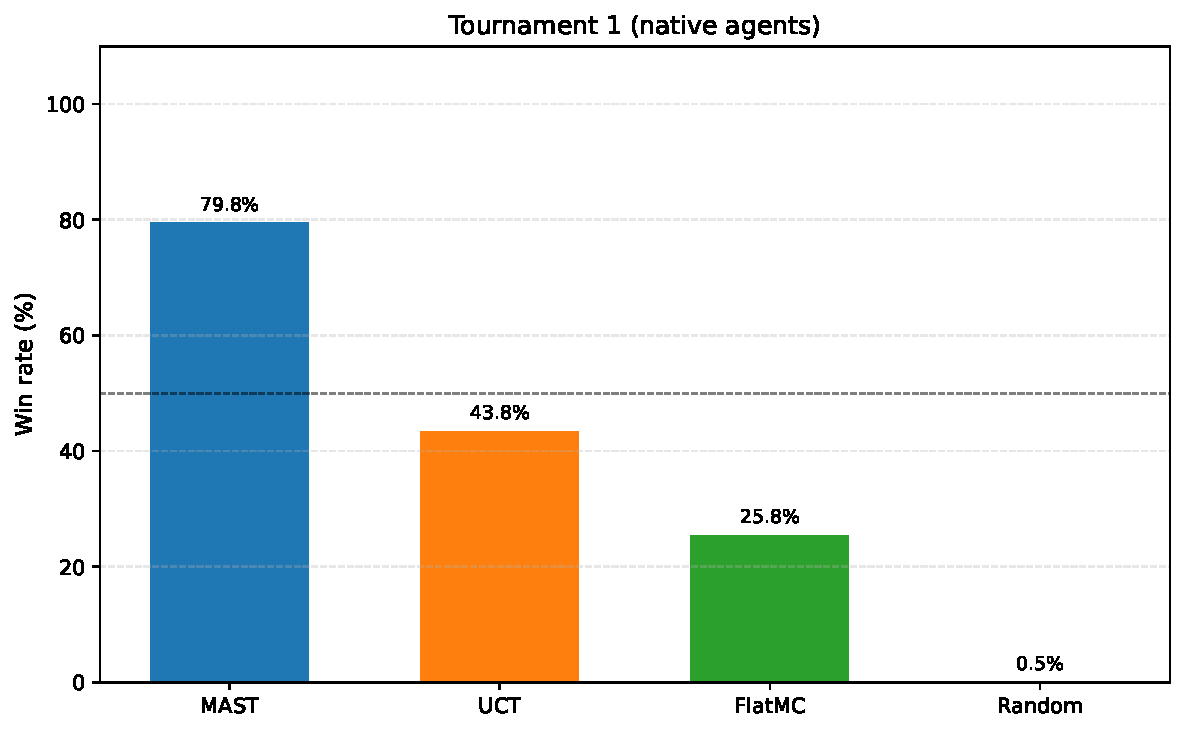
\includegraphics[width=\textwidth]{Sections/7_Results/figs/winrate_tournament_1_native_agents.pdf}
    \captionsetup{justification=centering}
    \caption{Win rates of native Ludii agents in Tournament 1. MAST, UCT, 
    and FlatMC achieve dramatically higher win rates than the Random agent, 
    confirming systematic access to hidden information through unrestricted 
    \texttt{copyContext()} calls. The near-zero win rate of Random (0.5\%) 
    reflects the fact that its opponents effectively play with perfect 
    information rather than reasoning under uncertainty.}
    \label{fig:ludii_t1_winrates}
\end{figure}

The results of Tournament 1 are unambiguous. MAST, UCT, and FlatMC all achieve dramatically higher win rates against the Random agent, while the Random agent performs at 0.5\% across all its matchups. MAST dominates the tournament with 99.8\%, followed by UCT at 58.5\% and FlatMC at 41.2\%.

This outcome is the direct empirical signature of the architectural 
problem identified in Chapter 4. Every \texttt{copyContext()} call 
made by MAST, UCT, or FlatMC during search returns a context 
containing the true positions of all opponent ships. The agent does 
not pursue a search strategy under uncertainty: it simply evaluates 
moves against the true board, which trivially reduces the game to a 
deterministic sequence of targeted shots. The Random agent, which 
never makes such calls, cannot access this information and therefore 
performs at near-zero level.

\newpage

\begin{figure}[H]
    \centering
    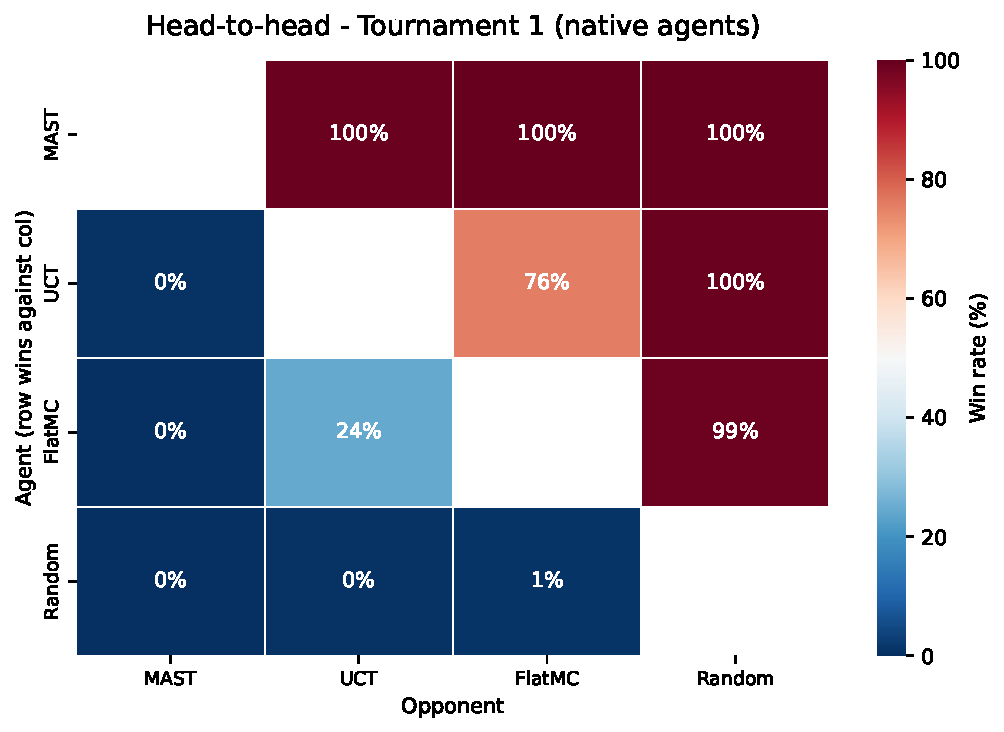
\includegraphics[width=\textwidth]{Sections/7_Results/figs/heatmap_tournament_1_native_agents.pdf}
    \captionsetup{justification=centering}
    \caption{Head-to-head win rates for native Ludii agents in Tournament 1. 
    MAST dominates every matchup, winning 100\% of its games against UCT, 
    FlatMC, and Random. All three search-based agents achieve near-perfect 
    win rates against Random (99--100\%), confirming that they exploit 
    privileged hidden-state information rather than reasoning under 
    uncertainty. Random wins virtually no games, consistent with opponents 
    playing with effective omniscience.}
    \label{fig:ludii_t1_heatmap}
\end{figure}

\subsection{Differences in Rollout Quality}

An additional observation concerns the relative performance of MAST, 
UCT, and FlatMC within Tournament 1. Since all three agents effectively play with full information due to the information leak, the stark contrast in their performance highlights how their respective rollout strategies exploit this unmasked state space. 

MAST's exceptional win rate (99.8\%) stems from its move-average statistics, which quickly converge toward the actual ship coordinates during simulations. Because the rollouts are executed on copies of the true, fully revealed game state, MAST's action-history table immediately identifies and prioritizes historically rewarded cells (hits), effectively guiding the simulation phases toward rapid victories. 

Conversely, UCT exploits the leaked state far less effectively (58.5\%). Without move-average statistics to bias its simulations, UCT relies on purely uniform random rollouts. These unguided rollouts dilute the critical feedback signal obtained from the unmasked root, as a sequence of random shots has an extremely low probability of stumbling into a winning configuration. This structural difference explains why UCT trails MAST so heavily despite both agents having full access to the board: its tree search cannot compensate for the noise introduced by its random rollout phase, whereas MAST transforms the leaked information into a highly effective simulation heuristic. FlatMC, which evaluates each action independently through flat rollouts, exploits the available information least efficiently of the three (41.2\%).

However, in a game where the true board is fully visible, even a 
single-step lookahead is sufficient to identify the optimal target 
at every turn: simply fire at any known ship cell. The performance 
gap between search-based agents in Tournament 1 therefore captures 
only second-order differences in sequential planning efficiency, not 
genuine strategic intelligence. The dominant effect remains 
information leakage.

\subsection{Confirmation of the Problem}

These results confirm the two key claims made in Chapter 4. First, 
the win-rate gap between simulation-based agents and the Random agent 
is entirely attributable to involuntary access to hidden information: 
no agent in this tournament is reasoning under uncertainty. Second, 
this gap renders all win-rate measurements for native Ludii agents 
in Battleship meaningless as evaluations of imperfect-information 
reasoning ability.


%%% 6.3 %%%
\section{Tournament 2: Determinized Agents}
\label{sec:tournament2}

\subsection{Results}

\begin{figure}[H]
    \centering
    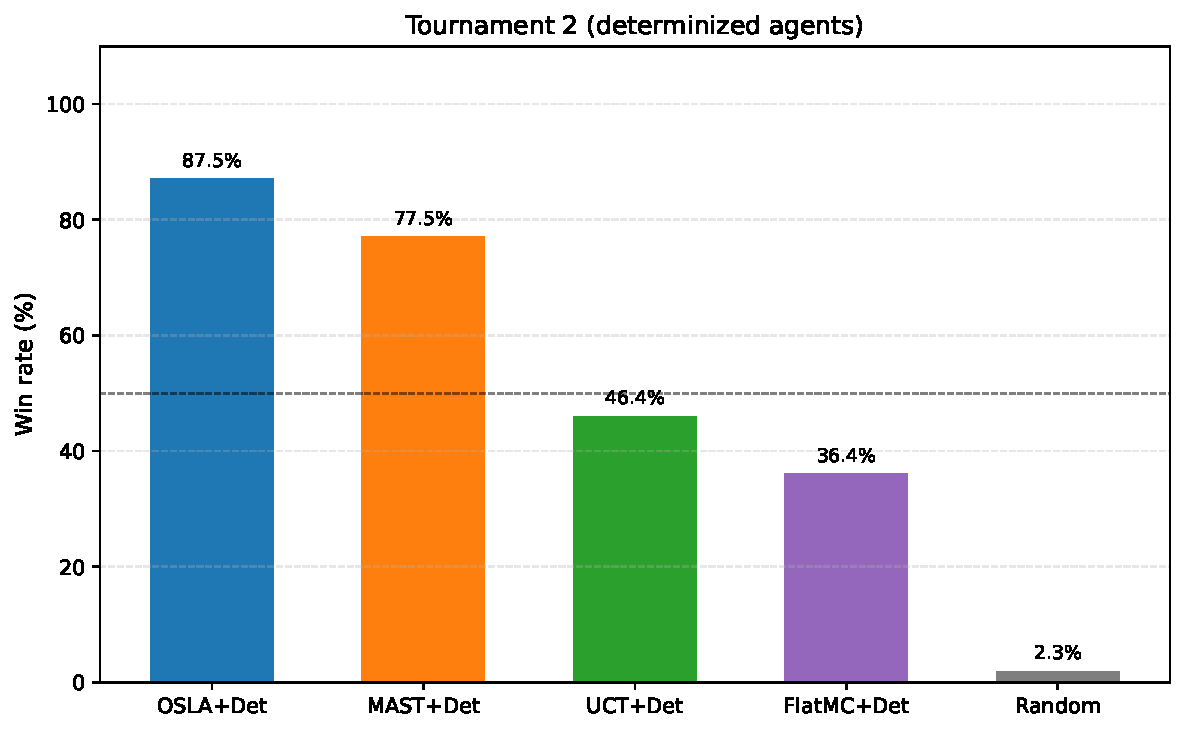
\includegraphics[width=\textwidth]{Sections/7_Results/figs/winrate_tournament_2_determinized_agents.pdf}
    \captionsetup{justification=centering}
    \caption{Win rates of determinized Ludii agents in Tournament 2. 
    OSLA+Det dominates at 87.5\%, closely matching its TAG counterpart, 
    followed by MAST+Det at 77.5\%. The information leakage advantage 
    observed in Tournament 1 is eliminated: Random recovers to 2.3\%, 
    consistent with agents now reasoning under genuine uncertainty rather 
    than exploiting privileged state information.}
    \label{fig:ludii_t2_winrates}
\end{figure}

The first and most important observation from Tournament 2 is that the artificial performance advantage observed in Tournament 1 is eliminated. The determinized agents no longer play with knowledge of the true ship positions; instead, each context copy they receive reflects a coherent hypothetical fleet consistent only with their own past observations. The signature of this change is twofold. First, the ordering of the agents now reflects search quality rather than raw access to the hidden state: OSLA+Det emerges as the strongest agent at 87.5\%, closely mirroring its performance in the TAG benchmark and confirming that the determinization layer provides a genuine and exploitable signal even for shallow one-step search. Second, the Random agent no longer collapses to near-zero: it recovers to 2.3\%, the level expected when its opponents must genuinely reason under uncertainty rather than fire directly at known ship cells. This 2.3\% closely matches the ~2\% observed for Random under Constraint-Based Determinization in TAG (Table 3.1), confirming that the Ludii determinization layer reproduces the leakage-free regime established in the reference benchmark.

This result validates the core claim of Chapter 5: the determinization 
layer correctly intercepts the raw context copy and replaces it with 
a coherent hypothesis, removing the privileged information that was 
available to native agents.

\begin{figure}[H]
    \centering
    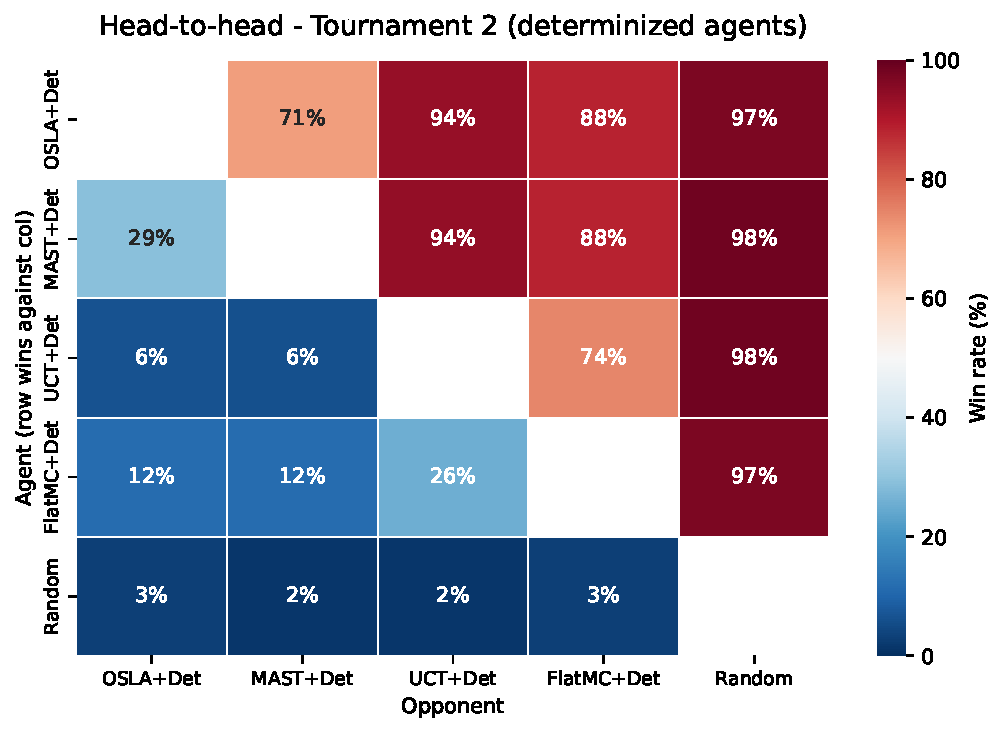
\includegraphics[width=\textwidth]{Sections/7_Results/figs/heatmap_tournament_2_determinized_agents.pdf}
    \captionsetup{justification=centering}
    \caption{Head-to-head win rates for determinized Ludii agents in 
    Tournament 2. OSLA+Det dominates with win rates of 71--97\% against 
    all opponents. MAST+Det also performs strongly, winning 88--98\% 
    against UCT+Det, FlatMC+Det, and Random. Random recovers to 2--3\% 
    against all agents, confirming that the information leakage advantage 
    has been eliminated and that performance differences now reflect 
    genuine reasoning under uncertainty.}
    \label{fig:ludii_t2_heatmap}
\end{figure}

\subsection{Relative Performance of Determinized Agents}

Within Tournament 2, meaningful differences in win rate emerge between 
the determinized agents. OSLA+Det leads at 87.5\%, followed by 
MAST+Det at 77.5\%, UCT+Det at 46.4\%, and FlatMC+Det at 36.4\%. 
These differences are interpretable as genuine reflections of search 
quality under uncertainty rather than artifacts of information leakage.

OSLA+Det and MAST+Det clearly outperform UCT+Det and FlatMC+Det. 
OSLA+Det benefits directly from coherent one-step hypotheses: at each 
decision step, it targets the cell that appears occupied in the 
determinized context, which is precisely the spatial reasoning that 
constraint-based filtering enables. MAST+Det accumulates move-average 
statistics across simulations performed on coherent hypothetical worlds, 
progressively reinforcing actions that target likely ship positions.

UCT+Det, by contrast, builds a search tree through repeated 
simulations but its rollout policy remains uniform random, limiting 
the value of deeper search. FlatMC+Det suffers from the same 
limitation without the benefit of tree construction. The performance 
ordering in Tournament 2 therefore mirrors the pattern observed in 
the Constraint-Based Determinization condition of Chapter 3: greedy 
and statistically-informed agents benefit most from coherent 
hypotheses, while tree-search agents are bottlenecked by rollout 
quality rather than search depth.

\subsection{Computational Overhead}

The Ludii evaluation does not provide per-copy timing metrics through 
the standard agent interface, so computational overhead cannot be 
quantified precisely in this setting. Qualitatively, determinized 
agents require substantially more wall-clock time per tournament than 
native agents, due to the history reconstruction and constraint-based 
hypothesis generation performed at each \texttt{copyContext()} call. 
This overhead is proportional to the number of moves already played 
and to the number of CSP placement attempts required before a valid 
configuration is found.

In practice, this overhead does not prevent search-based agents from 
completing a meaningful number of simulations within the 1000\,ms 
budget, as evidenced by the non-trivial win rates achieved by 
MAST+Det and OSLA+Det. However, it likely reduces the effective simulation count relative to native agents. The lower win rate of UCT+Det compared to native UCT should not be read as a regression caused by this overhead: native UCT played with full information, whereas UCT+Det reasons under genuine uncertainty and against a stronger, fully determinized field (including OSLA+Det). The two figures are therefore not directly comparable. 


%%% 6.4 %%%
\section{Comparison with the TAG Reference Benchmark}
\label{sec:comparison_tag}

\subsection{Structural Differences Between the Two Settings}

Before comparing results numerically, it is important to acknowledge the structural differences between the TAG and Ludii experimental settings. The agent populations differ: TAG used OSLA, RMHC, IS-MCTS, and MAST, while Ludii used UCT, MAST, 
FlatMC, and OSLA+Det (re-implemented from TAG). The framework implementations of shared algorithm families such as MCTS differ in their internal details. TAG provided three determinization strategies (Random, Constraint-Based, and Heatmap-Guided), while the Ludii determinization layer implements the Constraint-Based strategy only as its primary mode. These differences make a direct agent-by-agent comparison inappropriate. The comparison is therefore conducted at the level of behavioral patterns.

\subsection{Pattern 1: Convergence to Chance Under No Determinization}
The most fundamental prediction from Chapter~\ref{BattleshipInTAG} is that 
simulation-based agents given access to incoherent hidden states should not 
outperform the Random agent. Under Random Determinization in TAG, all agents 
performed near chance level, with win rates ranging from 44\% to 53\%, 
reflecting the absence of any useful signal in the incoherent hypotheses. 
Under native Ludii without the determinization layer, agents achieve 
near-perfect win rates against Random. It's not chance, but omniscience: they 
are not being given incoherent information, they are being given perfect 
information.

This asymmetry highlights that the Ludii native condition is not a form of 
Random Determinization but rather a form of omniscient play. Tournament~1 
therefore does not replicate the TAG Random Determinization condition; it 
represents a qualitatively different and more severe failure mode. The 
elimination of this information advantage is instead what Tournament~2 
demonstrates: once agents receive coherent hypotheses rather than the true 
hidden state, their performance reflects genuine reasoning quality under 
uncertainty rather than privileged access, consistent with the leakage-free 
baseline established in TAG.

\subsection{Pattern 2: Recovery Under Constraint-Based Determinization}
Chapter~\ref{BattleshipInTAG} showed that introducing constraint-based determinization produced a dramatic improvement against the Random agent for all simulation-based agents, with OSLA and RMHC in particular reaching overall win rates well above 50\%. Tournament 2 reproduces this pattern directly. OSLA+Det achieves 87.5\%, consistent with the 87\% observed in TAG under Constraint-Based Determinization, confirming that the behavioral recovery under informed determinization is not framework-specific but reflects a general property of simulation-based search under hidden information. The re-implementation of OSLA in Ludii therefore serves as a direct 
empirical bridge between the two frameworks, strengthening the cross-framework comparison beyond a purely qualitative alignment.

\subsection{Pattern 3: The Role of the Random Agent as Invariant Anchor}
Across all conditions in both TAG and Ludii, the Random agent is the one invariant. Because it never calls a simulation copy method, its behavior is entirely unaffected by what the copy mechanism returns. Its win rate should remain unaffected by the quality of the copy mechanism, since it never calls copyContext(). Its absolute win rate therefore reflects only the genuine strength of its opponents under each condition, not any information advantage.

This prediction holds across all five conditions: TAG Random Determinization (Random $\approx 44\%$), TAG Constraint-Based (Random $\approx 2\%$), TAG Heatmap-Guided (Random $\approx 2\%$), Ludii native agents (Random $\approx 0.5\%$), and Ludii determinized agents (Random $\approx 2.3\%$). The consistent behavior of the Random agent across frameworks and conditions provides strong evidence that the observed effects are due to the determinization mechanism rather than to confounding factors.


%%% 6.5 %%%
\section{Discussion and Limitations}
\label{sec:results_discussion}

\subsection{What the Results Establish}

The two Ludii tournaments together establish three things. The information leakage problem is real and measurable: native simulation-based Ludii agents play Battleship with effective omniscience, which fully accounts for their performance advantage over the Random agent. The determinization layer eliminates this advantage: once agents receive coherent hypothetical contexts rather than the true hidden state, their win rates fall back toward the levels expected under genuine uncertainty. And the behavioral patterns observed in Ludii after applying the determinization layer are qualitatively consistent with the TAG reference benchmark under Constraint-Based Determinization, validating the design of the solution across both frameworks.

\subsection{Limitations}

Several limitations should be acknowledged. The current evaluation is restricted to Battleship, a game with a particularly clean and well-defined hidden-information structure. Applying the determinization layer to other imperfect-information games in the Ludii library, such as Stratego or card games involving hidden identities, would require the extended \texttt{what}-field injection described in Section~\ref{sec:detect_hidden} as future work, and would introduce additional challenges in history reconstruction for games with more complex observation structures.

The constraint-based hypothesis generator can in principle fail to find a valid ship configuration within its allotted attempts, falling back to random placement. As discussed in Chapter~\ref{BattleshipInTAG}, this fallback rate is low in practice but non-zero. In the Ludii setting, the fallback has the additional effect of reintroducing random determinization for individual copy calls, slightly degrading the consistency of the information provided to the search algorithm.

Additionally, the history reconstruction mechanism in \newline
\texttt{BattleshipDeterminizationAgent} reads hit and miss 
outcomes after replaying the full move history from the Trial. 
While this correctly reconstructs the player's observations, 
the reconstruction is performed fresh at each decision step, 
introducing an overhead that grows linearly with game length. 
Maintaining an incremental observation log would substantially 
reduce this cost and constitutes a natural direction for 
optimization.

Finally, the comparison with TAG is strengthened by the re-implementation 
of OSLA+Det as a shared agent, but remains limited by the absence 
of RMHC and by differences in the internal implementations of 
UCT and MAST between the two frameworks. The qualitative alignment of behavioral patterns is encouraging, but a more rigorous cross-framework comparison would require either porting TAG agents to Ludii or re-implementing Ludii agents in TAG under identical computational conditions. This is left as a direction for future work.

\subsection{Summary}

The experimental evaluation confirms that the determinization layer proposed in Chapter~\ref{DeterminizationLayerLudii} achieves its primary objective: it transforms Ludii Battleship from a game in which simulation-based agents play with perfect information into one in which they reason under genuine uncertainty. The resulting behavioral patterns are consistent with the TAG reference benchmark, providing empirical support for the design and implementation of the solution. The limitations identified here, primarily the restriction to positional hidden information and the modest nature of the cross-framework comparison, outline the natural extensions of this work toward a more complete treatment of imperfect-information reasoning in general game playing systems.
